\section{Gestion de la documentation du projet}

La totalité de la documentation du projet sera hébérgé sur l'espace collaboratif GitHub.

GitHub met à disposition des membres de l'équipes, un dépot git afin de versionner les fichiers et de centraliser les modifications.
Chacun des membres de l’équipe auras donc accès à tout moment aux documents pour les éditer en ligne, ou hors ligne.

La production de document se fera à l’aide de LaTeX.

Chaque document, sera rangé dans un dossier contenant ses sources au format texte, les documents joints, le livrable au format pdf, ainsi qu'un  ainsi qu'un script \texttt{make} permettant de créer le livrable facilement.

L'arborescence d'un document type pourrait être :
\begin{description}
    \item[src]{Le dossier {\bf src} contient les fichiers textes composant le livreable.}
    \begin{description}
        \item[main.tex]{Le fichier {\bf main.tex} est le fichier principale du livreable, il contient toutes les informations relatives au document (titres, auteurs, dates ...).}
        \item[nation.tex] {Le fichier {\bf nation.tex} est inclus par {\bf main.tex} et contient les specifications de mise en forme du document final.}
        \item[satellite.tex] {Le fichier {\bf satellite.tex} est inclus par {\bf main.tex} et contient tout le corps du document. C'est ce fichier qui sera principalement édité par les membres de l'équipes}
    \end{description}
    \item [bin]{Le dossier {\bf bin} ne contient que le livreable au format pdf}
    \item [tmp]{Le dossier {\bf tmp} sert de dossier temporaire pour la compilation du document final. Il n'existe pas sur le dépôt commun.}
    \item [Makefile]{Le fichier {\bf Makefile} est un script permettant d'automatiser la génération du document.}
\end{description}

\section{Description de la mise en forme des documents}

\subsection{La mise en forme des documents sources}
    Pour assurer une meilleur relecture et compréhension des fichiers textes par tout les membres de l'équipe, quelques règles devront être appliqués :
    \begin{itemize}
        \item Le texte sera indenté en fonction de sont importance (section, sous section, sous sous section, paragraphe, sous paragraphe etc ...)
        \item Chaque niveau d'indentation se fera par 4 espaces.
        \item Ne pas hésiter à aérer le texte en passant à la ligne et en insérant des espaces de compréhension entre les commandes.
        \item Les règles de ponctuation du français devront être respecté.
    \end{itemize}

\subsection{La mise en forme des documents finaux}
La mise en forme finale des documents sera faite par LaTeX.
Ainsi elle sera parfaitement homogéne entre tous les documents, et certaines parties des documents pourront être automatisés.
Une tête de page sera affecté à chaque page du document excépté la page de garde, elle indiquera le titre du document.
Un pieds de page sera affecté à chaque page du document, il indiquera le numéro de page.

\subsection{Page de garde}

    La page de garde comportera :
    \begin{itemize}
      \item le titre.
      \item le numéro de l'hexanôme.
      \item les noms des auteurs sous la forme : Prénom \textsc{Nom}.
      \item la date de dernière mise à jour du document.
    \end{itemize}
    La première page de ce document peut servir d'exemple.
    Dans la pratique, la page de garde est décrite dans un fichier différent du corp du document, et est généré automatiquement à partir des informations ci-dessus.

\subsection{Sommaire}
  
   Le sommaire récapitule l'ensemble des pages où se trouvent les titres des sections, des sous sections et des sous sous sections.
   La numérotation des titres se fera en chiffre arabe, et un point séparera chaque niveau de numérotation.
   La page où se trouve le titre sera indiqué à droite.
   Un lien hypertexte permettra d'accéder à partir du sommaire, directement à l'ensemble des titres et sous titres.

\subsection{La numérotation}
   
   \subsubsection{titre de section}
   \begin{itemize}
        \item Numéro de la section
   \end{itemize}
        Exemple : 1

   \subsubsection{titre de sous section}
   \begin{itemize}
      \item Numéro de section parente
      \item Suivi d'un point
      \item Numéro de la sous section
   \end{itemize}
        Exemple : 1.2

   \subsubsection{titre de sous sous section}
   \begin{itemize}
      \item Numéro de section parente
      \item Suivi d'un point
      \item Numéro de la sous section
      \item Suivi d'un point
      \item Numéro de la sous sous section
   \end{itemize}
        Exemple : 1.2.4

\section{Le cycle de vie des documents}

\begin{center}
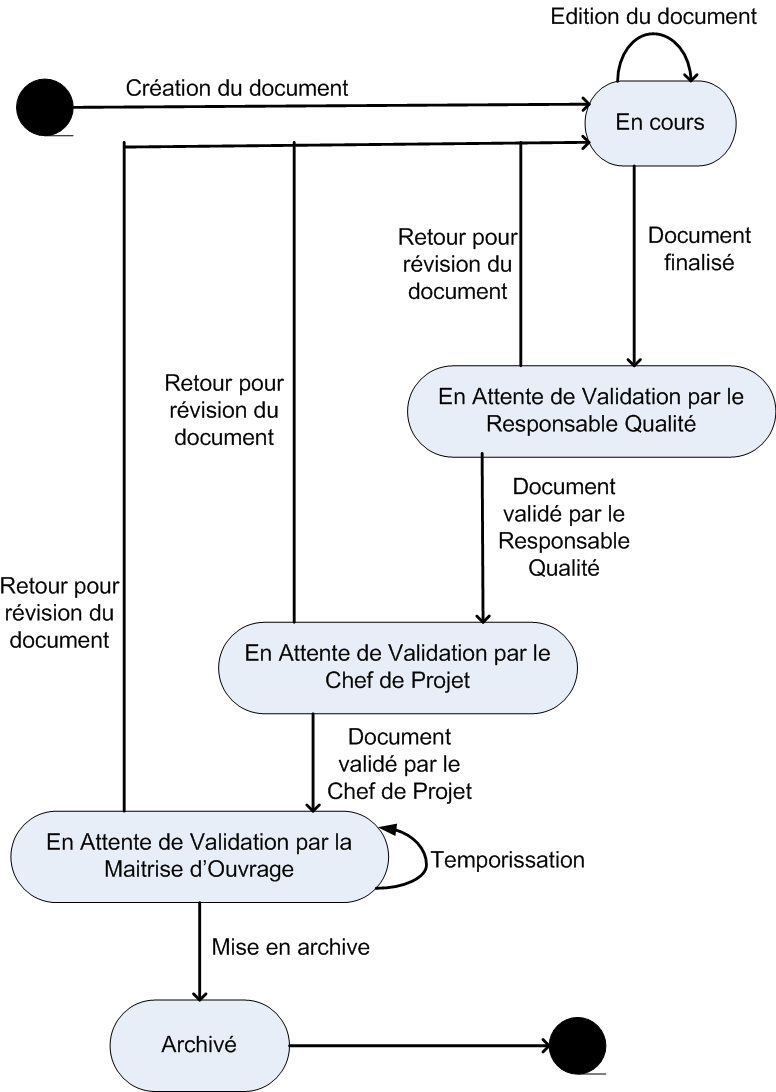
\includegraphics[width=0.6\textwidth]{img/cycleVie.png}
\end{center}

\section{La procédure interne de validation}

La validation interne des livrables se fera de manière continue, tout au long de sa rédaction.
Lorsque l’auteur juge avoir fini tout ou partie du document, il contacte le responsable qualité pour une première relecture. Le chef de projet pourras effectuer une seconde relecture.

Si des corrections sont à faire, deux solutions sont possibles.
En cas de corrections mineurs (fautes d’orthographes, quelques problèmes de présentations ...) la correction est effectué directement par le relecteur.
En cas de correction majeur (problème de fond, irrespect du modèle de présentation ...) une demande de correction sera envoyé à l’auteur soulevant un problème ou en laissant des commentaires dans le document.

Dans tout les cas, les relectures se feront le plus vite possible.
L’auteur doit prévoir dans sa rédaction le temps nécessaire à la relecture et la correction afin d’éviter les retard dans la livraison du document.

Les documents qu'on va réaliser passent dans plusieurs états au fur et à mesure de leur élaboration. Chaque document peut passer par plusieurs états selon son contenu. Voici les états possibles pour un document réalisé:

%TABLEAU A INSÉRER
%Le tableau est en ligne sur le google doc, dans le document nommé "paq",
%il se trouve dans le chapitre "La procédure interne de validation" de ce document.


\section{La procédure de recette client}

La procédure de validation du client pourras débuter à la date limite de rendu du livrable, sauf indication de retard. Le livrables sera déposé sur l'espace commun moodle dans la rubrique correspondante au document.

Si le client est dans l’incapacité de récupérer le document (document corrompu, introuvable ...) il peut prévenir par mail le responsable communication afin que l’équipe puisse redéposer le livrable.
Si moodle devenait inutilisable, les documents seraient livrés au client par mail temporairement.

Une fois le document en possession du client, la relecture pourra prendre jusqu’à une semaine.

En cas de non-validation, le client pourras contacter par mail ou pendant une réunion le responsable communication ou le chef d’équipe afin qu’il fasse remonter les remarques au reste de l’équipe.
Il sera en charge de formuler les réclamation de manière compréhensible.

En cas de correction à apporter au document, cette correction pourra être livré en 3 jours.
Nous serons chargé de prévenir le client de la livraison d’une correction.

\section{Les outils utilisés durant le projet}

La gestion de la documentation se fera à l’aide de l’outil Git, hébergé sur le site GitHub.
GitHub pourras être utilisé pour remonter tout type de problème concernant la documentation, et ainsi suivre l'évolution et la discussion autour du problème.
GitHub permettant de versionner les fichiers, il sera facile de suivre l'évolution de la production du document.
Chaque auteur, après une modification devras écrire un court commentaire concernant sa modification.
Il sera également facile de remonter les modifications et de réparer les erreurs très rapidement.

La rédaction de document se fera à l’aide de n’importe quel éditeur de texte, ou de l'outils en ligne proposé par GitHub.
La production de la documentation se fera à l’aide de l'outil LaTeX.

Pour augmenter l'efficacité de l'équipe sur le projet, l’idéal est de minimiser le cycle de vie des documents.
C'est pour cette raison que LaTeX à été choisi pour produire les documents. Ainsi, le temps de mise en page qui peut être long et fastidieux est économisé.

Cette solution permettras à chacun  d’utiliser ces outils habituels d’éditions de textes, tout en assurant une cohérence parfaite entre les documents.

\section{ANNEXES}
\begin{description}
\item[Annexe 1 : Exemple de la page de garde]
    {Insérer Modèle}
\item[Annexe 2 : Fiche de suivi individuel par séance]
    Insérer Modèle
\item[Annexe 3 : Fiche global de suivi]
    Insérer Modèle
\item[Annexe 4 : Fiche de suivi d'avancement des livrables]
    Insérer Modèle
\item[Annexe 5 : Journal de réunions]
    Modèle
\item[Annexe 6 : Tableau de bord d'avancement]
    Insérer Modèle
\end{description}
